\section{The Serial Safety Net}
%Das Serial Safety Net baut auf bestehenden Multiversion-Concurrency-Control-Verfahren auf, wobei es einen kreisfreien Abhängigkeitsgraphen und somit Serialisierbarkeit gewährleistet.
%Das zugrundeliegende Verfahren muss dabei mindestens das Isolationslevel Read Committed unterstützen.
Das Serial Safety Net baut auf bestehenden Multiversion-Concurrency-Control-Verfahren auf.
In einem System, welches Multiversion-Concurrency-Control(MVCC) verwendet, bestehen alle Datenbankelemente aus einer Sequenz von Versionen, wobei Schreiboperationen jeweils eine Version anlegen und Leseoperationen eine Version zurückgeben.

Für solche MVCC-Verfahren sichert das Serial Safety Net einen kreisfreien Abhängigkeitsgraphen, wodurch die Serialisierbarkeit des Transaktionsplans gewährleistet wird.
Der Abhängigkeitsgraph stellt dabei eine Übersicht über die Abhängigkeit zwischen den Transaktionen eines Plans dar, wobei die Knoten des Graphen die committeten Transaktionen und die Kanten die Abhängigkeiten zwischen diesen darstellen.
Ein Graph ohne Zyklen garantiert dabei immer, dass ein äquivalenter serieller Plan zu den ausgeführten Transaktionen existiert, welcher zum selben Ergebnis geführt hätte.

\begin{Definition}
	Die Abhängigkeit $T\leftarrow U$ zwischen den Transaktionen $T$ und $U$ besagt, dass $U$ von $T$ abhängig ist und somit $T$ als direkter Vorgänger und $U$ als direkter Nachfolger bezeichnet wird.
\end{Definition}

Eine zentrale Rolle bei der Umsetzung des Serial Safety Nets spielt die Untersuchung der Abhängigkeiten von Transaktionen in Verbindung mit der Commit-Reihenfolge.
Dazu lassen sich zwei verschiedene Typen von Abhängigkeiten wie folgt definieren.

\begin{Definition}
	Bei einer \textcolor{my-green}{Back-Edge} $T\xleftarrow{b} U$ committet der Nachfolger $U$ zuerst.
\end{Definition}

\begin{Definition}
	Bei einer \textcolor{my-blue}{Forward-Edge} $T\xleftarrow{f} U$ committet der Vorgänger $T$ zuerst.
\end{Definition}

\begin{Definition}
	Eine reflexive, transitive \textcolor{my-green}{Back-Edge} $T\xleftarrow{b*} U$ bezeichnet eine Verbindung, bei der $T$ von $U$ ausschließlich über Back-Edges erreichbar ist.
\end{Definition}

\begin{figure}
	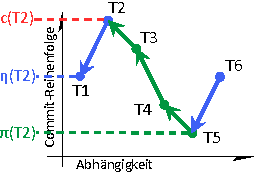
\includegraphics{img/Figure_2_1.pdf}
	\caption{Veranschaulichung von \textcolor{my-green}{Back}- und \textcolor{my-blue}{Forward-Edges} sowie den Zeitstempeln von Transaktion $T2$}
	\label{fig:back_forward}
\end{figure}

Zum besseren Verständnis sind die genannten Begriffe in Abbildung \ref{fig:back_forward} veranschaulicht worden.
Die abgebildeten Back-Edges ergeben zusammen eine reflexive, transitive Back-Edge von Transaktion $T2$ zu $T5$.

Die Umsetzung des Serial Safety Nets erfordert das Erfassen der folgenden drei Zeitstempel zu jeder Transaktion, welche es später erlauben einen Abhängigkeitszyklus zu erkennen.
Die vorgestellten Zeitstempel sind ebenfalls in Abbildung \ref{fig:back_forward} für die Transaktion $T2$ eingezeichnet.

\begin{Definition}
	\textcolor{my-red}{$c(T)$} bezeichnet die Commit-Zeit der Transaktion $T$
\end{Definition}

\begin{Definition}
	\textcolor{my-green}{$\pi (T)$} bezeichnet die Commit-Zeit des ältesten Nachfolgers, der durch Back-Edges erreichbar ist:\\		
	$\pi (T)=\min (c(U):T\xleftarrow{b*}U)=\min (\{\pi (U):T\xleftarrow{b}U\}\cup \{c(T)\})$
\end{Definition}

\begin{Definition}
	\textcolor{my-blue}{$\eta (T)$} bezeichnet die Commit-Zeit des zuletzt committeten Vorgängers von $T$:\\
	$\eta (T) = \max (\{c(U):U\xleftarrow{f} T\}\cup \{-\infty \})$
\end{Definition}
